\documentclass{standalone}
\usepackage{tikz}
\usetikzlibrary{patterns, positioning}
\usepackage[sfdefault]{ClearSans} %% option 'sfdefault' activates Clear Sans as the default text font
\usepackage[T1]{fontenc}

\begin{document}
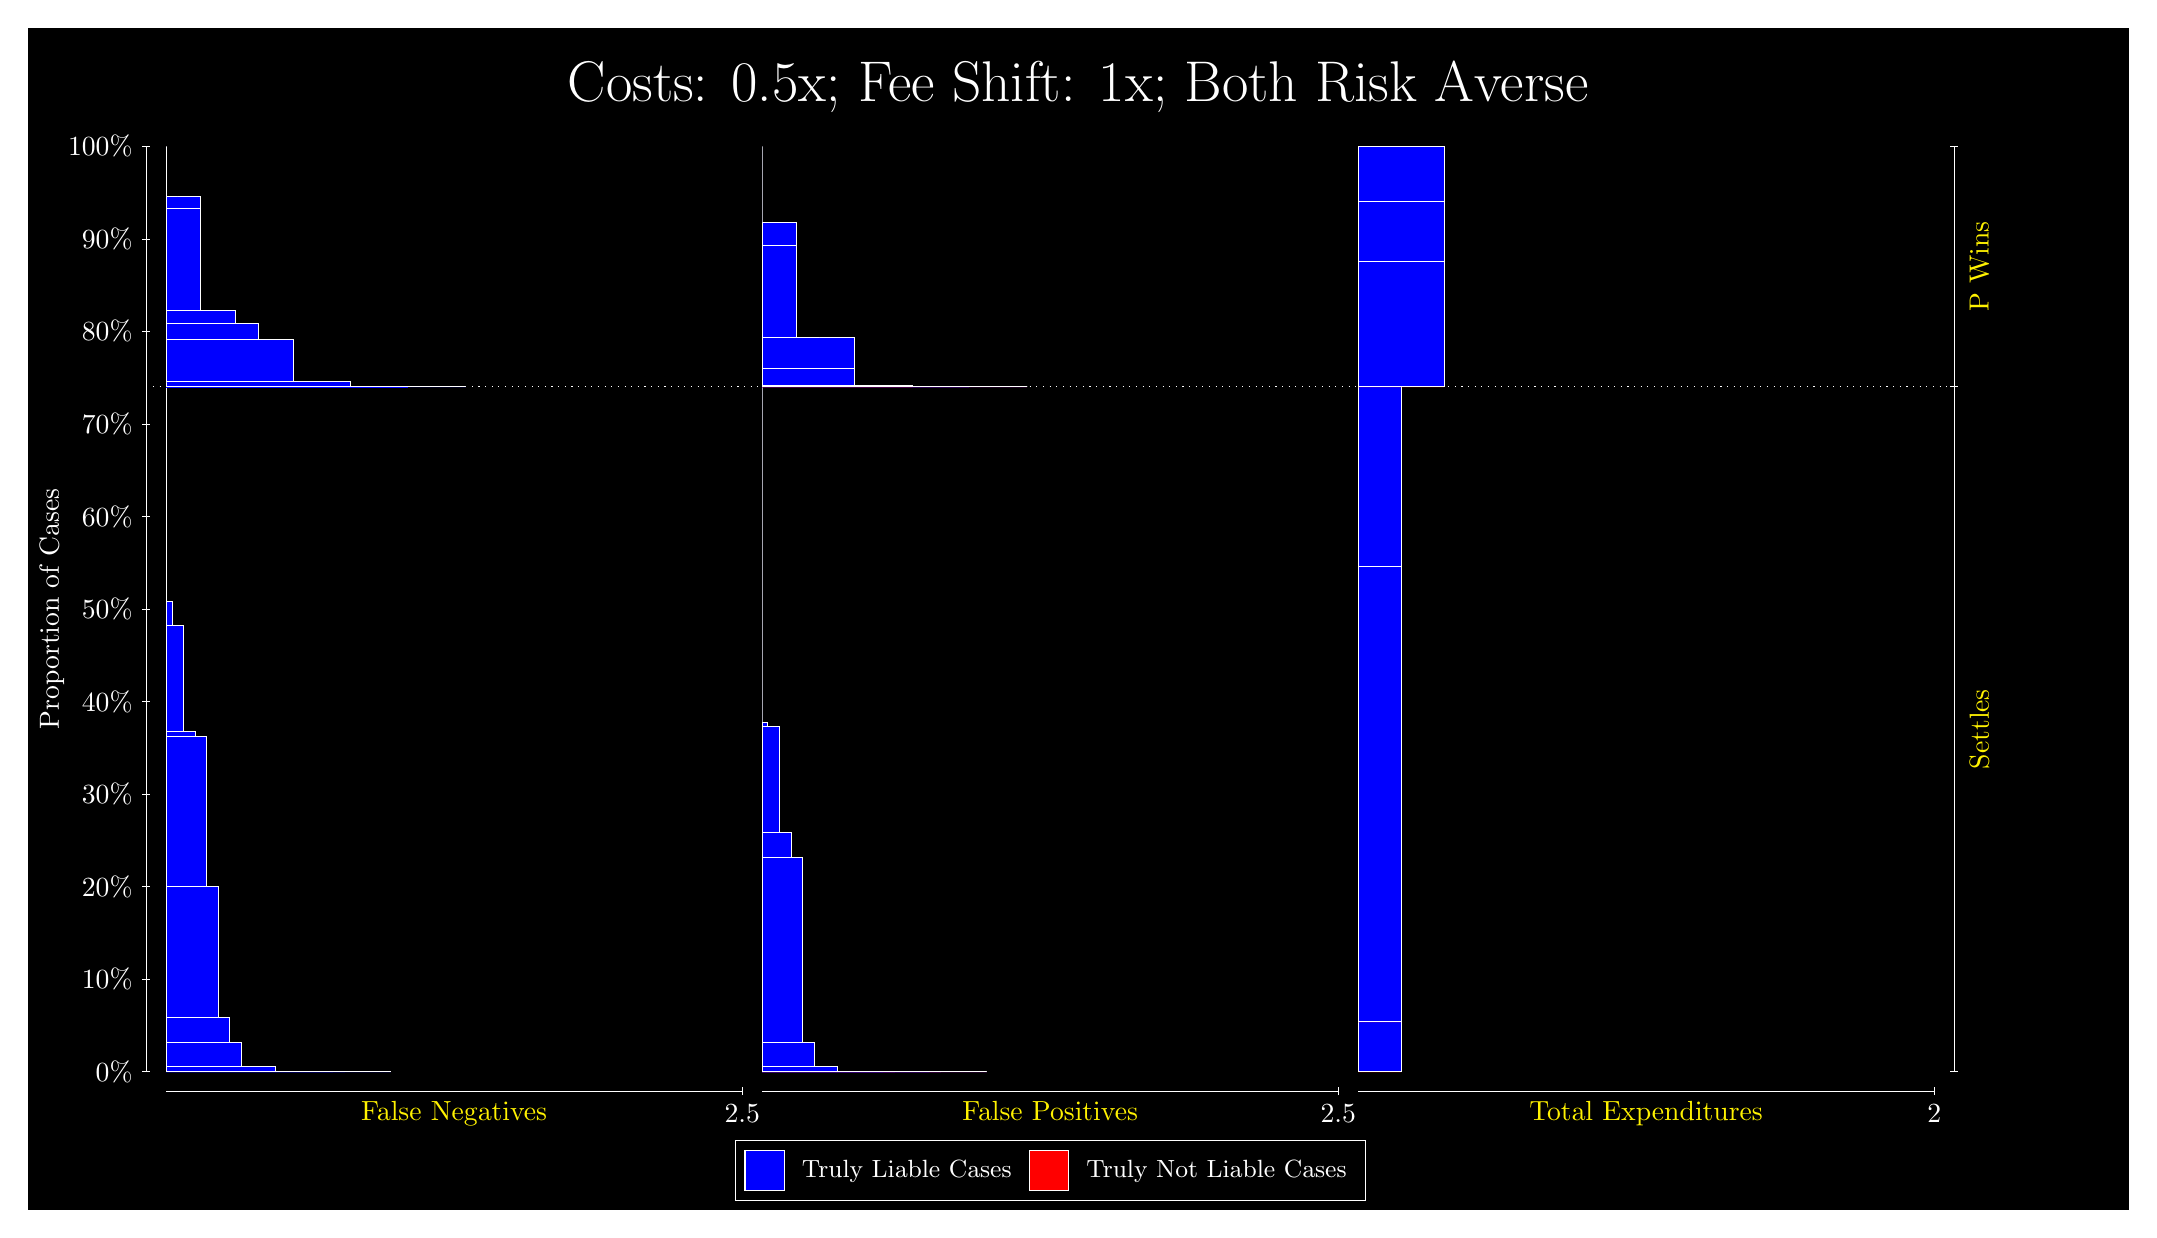
\begin{tikzpicture}
\draw[fill=black] (0,0) rectangle (26.667,15);
\draw[text=white] (0,13.5) rectangle (26.667,15) node[midway] {\huge Costs: 0.5x; Fee Shift: 1x; Both Risk Averse};
\draw[white, very thin] (1.5,1.75) -- (1.5,13.5);
\node[rotate=90, text=white, anchor=center] at (0.3, 7.625) {Proportion of Cases};
\draw[white, very thin] (1.45,1.75) -- (1.55,1.75);
\node[text=white, anchor=east] at (1.45, 1.75) {0\%};
\draw[white, very thin] (1.45,2.925) -- (1.55,2.925);
\node[text=white, anchor=east] at (1.45, 2.925) {10\%};
\draw[white, very thin] (1.45,4.1) -- (1.55,4.1);
\node[text=white, anchor=east] at (1.45, 4.1) {20\%};
\draw[white, very thin] (1.45,5.275) -- (1.55,5.275);
\node[text=white, anchor=east] at (1.45, 5.275) {30\%};
\draw[white, very thin] (1.45,6.45) -- (1.55,6.45);
\node[text=white, anchor=east] at (1.45, 6.45) {40\%};
\draw[white, very thin] (1.45,7.625) -- (1.55,7.625);
\node[text=white, anchor=east] at (1.45, 7.625) {50\%};
\draw[white, very thin] (1.45,8.8) -- (1.55,8.8);
\node[text=white, anchor=east] at (1.45, 8.8) {60\%};
\draw[white, very thin] (1.45,9.975) -- (1.55,9.975);
\node[text=white, anchor=east] at (1.45, 9.975) {70\%};
\draw[white, very thin] (1.45,11.15) -- (1.55,11.15);
\node[text=white, anchor=east] at (1.45, 11.15) {80\%};
\draw[white, very thin] (1.45,12.325) -- (1.55,12.325);
\node[text=white, anchor=east] at (1.45, 12.325) {90\%};
\draw[white, very thin] (1.45,13.5) -- (1.55,13.5);
\node[text=white, anchor=east] at (1.45, 13.5) {100\%};

\draw[white, very thin] (24.457,1.75) -- (24.457,13.5);
\draw[white, very thin] (24.407,1.75) -- (24.507,1.75);
\node[anchor=west] at (24.407, 1.75) {};
\draw[white, very thin] (24.407,10.447) -- (24.507,10.447);
\node[anchor=west] at (24.407, 10.447) {};
\draw[white, very thin] (24.407,13.5) -- (24.507,13.5);
\node[anchor=west] at (24.407, 13.5) {};

\draw[white, very thin, fill=blue] (1.75,1.75) rectangle (4.6044,1.75);
\draw[white, very thin, fill=blue] (1.75,1.75) rectangle (4.0188,1.75);
\draw[white, very thin, fill=blue] (1.75,1.75) rectangle (3.8725,1.75);
\draw[white, very thin, fill=blue] (1.75,1.75) rectangle (3.4333,1.7507);
\draw[white, very thin, fill=blue] (1.75,1.7507) rectangle (3.287,1.7534);
\draw[white, very thin, fill=blue] (1.75,1.7534) rectangle (3.1406,1.8125);
\draw[white, very thin, fill=blue] (1.75,1.8125) rectangle (2.8478,1.8156);
\draw[white, very thin, fill=blue] (1.75,1.8156) rectangle (2.7015,2.1275);
\draw[white, very thin, fill=blue] (1.75,2.1275) rectangle (2.5551,2.4407);
\draw[white, very thin, fill=blue] (1.75,2.4407) rectangle (2.4087,4.1033);
\draw[white, very thin, fill=blue] (1.75,4.1033) rectangle (2.2623,6.007);
\draw[white, very thin, fill=blue] (1.75,6.007) rectangle (2.1159,6.0654);
\draw[white, very thin, fill=blue] (1.75,6.0654) rectangle (1.9696,7.4135);
\draw[white, very thin, fill=blue] (1.75,7.4135) rectangle (1.8232,7.7275);
\draw[white, very thin, fill=red] (1.75,7.7275) rectangle (1.75,7.7275);
\draw[white, very thin, fill=blue] (1.75,7.7275) rectangle (1.75,10.447);
\draw[white, very thin, fill=blue] (1.75,10.447) rectangle (5.5558,10.447);
\draw[white, very thin, fill=blue] (1.75,10.447) rectangle (4.8239,10.448);
\draw[white, very thin, fill=blue] (1.75,10.448) rectangle (4.3848,10.448);
\draw[white, very thin, fill=blue] (1.75,10.448) rectangle (4.092,10.513);
\draw[white, very thin, fill=blue] (1.75,10.513) rectangle (3.6529,10.513);
\draw[white, very thin, fill=blue] (1.75,10.513) rectangle (3.3602,11.05);
\draw[white, very thin, fill=blue] (1.75,11.05) rectangle (2.921,11.259);
\draw[white, very thin, fill=blue] (1.75,11.259) rectangle (2.6283,11.416);
\draw[white, very thin, fill=blue] (1.75,11.416) rectangle (2.1891,12.709);
\draw[white, very thin, fill=blue] (1.75,12.709) rectangle (2.1891,12.868);
\draw[white, very thin, fill=blue] (1.75,12.868) rectangle (1.8964,12.868);
\draw[white, very thin, fill=red] (1.75,12.868) rectangle (1.75,12.868);
\draw[white, very thin, fill=blue] (1.75,12.868) rectangle (1.75,13.5);
\draw[white, very thin, fill=red] (9.3189,1.75) rectangle (12.173,1.75);
\draw[white, very thin, fill=blue] (9.3189,1.75) rectangle (12.173,1.75);
\draw[white, very thin, fill=red] (9.3189,1.75) rectangle (11.588,1.75);
\draw[white, very thin, fill=blue] (9.3189,1.75) rectangle (11.588,1.75);
\draw[white, very thin, fill=blue] (9.3189,1.75) rectangle (11.441,1.75);
\draw[white, very thin, fill=red] (9.3189,1.75) rectangle (11.002,1.75);
\draw[white, very thin, fill=blue] (9.3189,1.75) rectangle (11.002,1.75);
\draw[white, very thin, fill=blue] (9.3189,1.75) rectangle (10.856,1.75);
\draw[white, very thin, fill=blue] (9.3189,1.75) rectangle (10.709,1.7505);
\draw[white, very thin, fill=red] (9.3189,1.7505) rectangle (10.417,1.7505);
\draw[white, very thin, fill=blue] (9.3189,1.7505) rectangle (10.417,1.7543);
\draw[white, very thin, fill=blue] (9.3189,1.7543) rectangle (10.27,1.8131);
\draw[white, very thin, fill=blue] (9.3189,1.8131) rectangle (10.124,1.8152);
\draw[white, very thin, fill=blue] (9.3189,1.8152) rectangle (9.9776,2.1266);
\draw[white, very thin, fill=red] (9.3189,2.1266) rectangle (9.8312,2.1266);
\draw[white, very thin, fill=blue] (9.3189,2.1266) rectangle (9.8312,4.4691);
\draw[white, very thin, fill=blue] (9.3189,4.4691) rectangle (9.6848,4.7831);
\draw[white, very thin, fill=blue] (9.3189,4.7831) rectangle (9.5384,6.1313);
\draw[white, very thin, fill=blue] (9.3189,6.1313) rectangle (9.3921,6.1896);
\draw[white, very thin, fill=blue] (9.3189,6.1896) rectangle (9.3189,10.447);
\draw[white, very thin, fill=red] (9.3189,10.447) rectangle (12.686,10.447);
\draw[white, very thin, fill=blue] (9.3189,10.447) rectangle (12.686,10.447);
\draw[white, very thin, fill=red] (9.3189,10.447) rectangle (11.954,10.447);
\draw[white, very thin, fill=blue] (9.3189,10.447) rectangle (11.954,10.447);
\draw[white, very thin, fill=blue] (9.3189,10.447) rectangle (11.954,10.447);
\draw[white, very thin, fill=red] (9.3189,10.447) rectangle (11.222,10.447);
\draw[white, very thin, fill=blue] (9.3189,10.447) rectangle (11.222,10.454);
\draw[white, very thin, fill=blue] (9.3189,10.454) rectangle (11.222,10.468);
\draw[white, very thin, fill=red] (9.3189,10.468) rectangle (10.783,10.468);
\draw[white, very thin, fill=blue] (9.3189,10.468) rectangle (10.783,10.468);
\draw[white, very thin, fill=red] (9.3189,10.468) rectangle (10.49,10.468);
\draw[white, very thin, fill=blue] (9.3189,10.468) rectangle (10.49,10.687);
\draw[white, very thin, fill=blue] (9.3189,10.687) rectangle (10.49,11.079);
\draw[white, very thin, fill=red] (9.3189,11.079) rectangle (10.051,11.079);
\draw[white, very thin, fill=blue] (9.3189,11.079) rectangle (10.051,11.079);
\draw[white, very thin, fill=blue] (9.3189,11.079) rectangle (9.758,12.237);
\draw[white, very thin, fill=blue] (9.3189,12.237) rectangle (9.758,12.53);
\draw[white, very thin, fill=red] (9.3189,12.53) rectangle (9.3189,12.53);
\draw[white, very thin, fill=blue] (9.3189,12.53) rectangle (9.3189,13.5);
\draw[white, very thin, fill=red] (16.888,1.75) rectangle (17.437,1.75);
\draw[white, very thin, fill=blue] (16.888,1.75) rectangle (17.437,2.3837);
\draw[white, very thin, fill=red] (16.888,2.3837) rectangle (17.437,2.3837);
\draw[white, very thin, fill=blue] (16.888,2.3837) rectangle (17.437,8.1675);
\draw[white, very thin, fill=red] (16.888,8.1675) rectangle (17.437,8.1675);
\draw[white, very thin, fill=blue] (16.888,8.1675) rectangle (17.437,10.447);
\draw[white, very thin, fill=red] (16.888,10.447) rectangle (17.986,10.447);
\draw[white, very thin, fill=blue] (16.888,10.447) rectangle (17.986,12.04);
\draw[white, very thin, fill=red] (16.888,12.04) rectangle (17.986,12.04);
\draw[white, very thin, fill=blue] (16.888,12.04) rectangle (17.986,12.801);
\draw[white, very thin, fill=red] (16.888,12.801) rectangle (17.986,12.801);
\draw[white, very thin, fill=blue] (16.888,12.801) rectangle (17.986,13.5);
\draw[white, dotted] (1.5,10.447) -- (24.457,10.447);
\draw[white, very thin] (1.75,1.5) -- (9.0689,1.5);
\node[text=yellow, anchor=north] at (5.4094, 1.5) {False Negatives};
\draw[white, very thin] (9.0689,1.45) -- (9.0689,1.55);
\node[text=white, anchor=north] at (9.0689, 1.45) {2.5};

\draw[white, very thin] (9.3189,1.5) -- (16.638,1.5);
\node[text=yellow, anchor=north] at (12.978, 1.5) {False Positives};
\draw[white, very thin] (16.638,1.45) -- (16.638,1.55);
\node[text=white, anchor=north] at (16.638, 1.45) {2.5};

\draw[white, very thin] (16.888,1.5) -- (24.207,1.5);
\node[text=yellow, anchor=north] at (20.547, 1.5) {Total Expenditures};
\draw[white, very thin] (24.207,1.45) -- (24.207,1.55);
\node[text=white, anchor=north] at (24.207, 1.45) {2};

\node[text=yellow, centered, rotate=90] at (24.777, 6.0983) {Settles};
\node[text=yellow, centered, rotate=90] at (24.777, 11.973) {P Wins};

\draw (12.978300999999998,1.5) node[draw=none] (baseCoordinate) {};
\begin{scope}[align=center]
        \matrix[scale=0.5, draw=white, below=0.5cm of baseCoordinate, nodes={draw}, column sep=0.1cm]{
            \node[rectangle, draw, minimum width=0.5cm, minimum height=0.5cm, fill=blue] {}; &
            \node[draw=none, font=\small, text=white] (B) {Truly Liable Cases}; &
            \node[rectangle, draw, minimum width=0.5cm, minimum height=0.5cm, fill=red] {}; &
            \node[draw=none, font=\small, text=white] (B) {Truly Not Liable Cases}; \\
            };
\end{scope}

\end{tikzpicture}
\end{document}